\documentclass[10pt]{article} % For LaTeX2e

% This template and styling file have been adapted from the ML Reproducibility Challenge 2020 and TMLR templates, to ease the submission.

% If you want to show the general instuctions, use the following command:
\usepackage[instructions]{atml}
% For the final version, use this one:
%\usepackage{atml}

% If you want to submit this work to tmlr, use the "tmlr" package rather than the "atml" one. Note: double-check the files needed in TMLR's submission instructions. 
% \usepackage{tmlr}
% If accepted, instead use the following line for the camera-ready submission:
%\usepackage[accepted]{tmlr}
% To de-anonymize and remove mentions to TMLR (for example for posting to preprint servers), instead use the following:
%\usepackage[preprint]{tmlr}

% Note that the following lines have been added to atml.sty:
% \usepackage[hidelinks]{hyperref}
% \newcommand*{\doi}[1]{\href{http://doi.org/#1}{doi: #1}}
% If atml.sty is not used, then these lines might need to be added to the respective styling files.
%%%%% NEW MATH DEFINITIONS %%%%%

\usepackage{amsmath,amsfonts,bm}

% Mark sections of captions for referring to divisions of figures
\newcommand{\figleft}{{\em (Left)}}
\newcommand{\figcenter}{{\em (Center)}}
\newcommand{\figright}{{\em (Right)}}
\newcommand{\figtop}{{\em (Top)}}
\newcommand{\figbottom}{{\em (Bottom)}}
\newcommand{\captiona}{{\em (a)}}
\newcommand{\captionb}{{\em (b)}}
\newcommand{\captionc}{{\em (c)}}
\newcommand{\captiond}{{\em (d)}}

% Highlight a newly defined term
\newcommand{\newterm}[1]{{\bf #1}}


% Figure reference, lower-case.
\def\figref#1{figure~\ref{#1}}
% Figure reference, capital. For start of sentence
\def\Figref#1{Figure~\ref{#1}}
\def\twofigref#1#2{figures \ref{#1} and \ref{#2}}
\def\quadfigref#1#2#3#4{figures \ref{#1}, \ref{#2}, \ref{#3} and \ref{#4}}
% Section reference, lower-case.
\def\secref#1{section~\ref{#1}}
% Section reference, capital.
\def\Secref#1{Section~\ref{#1}}
% Reference to two sections.
\def\twosecrefs#1#2{sections \ref{#1} and \ref{#2}}
% Reference to three sections.
\def\secrefs#1#2#3{sections \ref{#1}, \ref{#2} and \ref{#3}}
% Reference to an equation, lower-case.
\def\eqref#1{equation~\ref{#1}}
% Reference to an equation, upper case
\def\Eqref#1{Equation~\ref{#1}}
% A raw reference to an equation---avoid using if possible
\def\plaineqref#1{\ref{#1}}
% Reference to a chapter, lower-case.
\def\chapref#1{chapter~\ref{#1}}
% Reference to an equation, upper case.
\def\Chapref#1{Chapter~\ref{#1}}
% Reference to a range of chapters
\def\rangechapref#1#2{chapters\ref{#1}--\ref{#2}}
% Reference to an algorithm, lower-case.
\def\algref#1{algorithm~\ref{#1}}
% Reference to an algorithm, upper case.
\def\Algref#1{Algorithm~\ref{#1}}
\def\twoalgref#1#2{algorithms \ref{#1} and \ref{#2}}
\def\Twoalgref#1#2{Algorithms \ref{#1} and \ref{#2}}
% Reference to a part, lower case
\def\partref#1{part~\ref{#1}}
% Reference to a part, upper case
\def\Partref#1{Part~\ref{#1}}
\def\twopartref#1#2{parts \ref{#1} and \ref{#2}}

\def\ceil#1{\lceil #1 \rceil}
\def\floor#1{\lfloor #1 \rfloor}
\def\1{\bm{1}}
\newcommand{\train}{\mathcal{D}}
\newcommand{\valid}{\mathcal{D_{\mathrm{valid}}}}
\newcommand{\test}{\mathcal{D_{\mathrm{test}}}}

\def\eps{{\epsilon}}


% Random variables
\def\reta{{\textnormal{$\eta$}}}
\def\ra{{\textnormal{a}}}
\def\rb{{\textnormal{b}}}
\def\rc{{\textnormal{c}}}
\def\rd{{\textnormal{d}}}
\def\re{{\textnormal{e}}}
\def\rf{{\textnormal{f}}}
\def\rg{{\textnormal{g}}}
\def\rh{{\textnormal{h}}}
\def\ri{{\textnormal{i}}}
\def\rj{{\textnormal{j}}}
\def\rk{{\textnormal{k}}}
\def\rl{{\textnormal{l}}}
% rm is already a command, just don't name any random variables m
\def\rn{{\textnormal{n}}}
\def\ro{{\textnormal{o}}}
\def\rp{{\textnormal{p}}}
\def\rq{{\textnormal{q}}}
\def\rr{{\textnormal{r}}}
\def\rs{{\textnormal{s}}}
\def\rt{{\textnormal{t}}}
\def\ru{{\textnormal{u}}}
\def\rv{{\textnormal{v}}}
\def\rw{{\textnormal{w}}}
\def\rx{{\textnormal{x}}}
\def\ry{{\textnormal{y}}}
\def\rz{{\textnormal{z}}}

% Random vectors
\def\rvepsilon{{\mathbf{\epsilon}}}
\def\rvtheta{{\mathbf{\theta}}}
\def\rva{{\mathbf{a}}}
\def\rvb{{\mathbf{b}}}
\def\rvc{{\mathbf{c}}}
\def\rvd{{\mathbf{d}}}
\def\rve{{\mathbf{e}}}
\def\rvf{{\mathbf{f}}}
\def\rvg{{\mathbf{g}}}
\def\rvh{{\mathbf{h}}}
\def\rvu{{\mathbf{i}}}
\def\rvj{{\mathbf{j}}}
\def\rvk{{\mathbf{k}}}
\def\rvl{{\mathbf{l}}}
\def\rvm{{\mathbf{m}}}
\def\rvn{{\mathbf{n}}}
\def\rvo{{\mathbf{o}}}
\def\rvp{{\mathbf{p}}}
\def\rvq{{\mathbf{q}}}
\def\rvr{{\mathbf{r}}}
\def\rvs{{\mathbf{s}}}
\def\rvt{{\mathbf{t}}}
\def\rvu{{\mathbf{u}}}
\def\rvv{{\mathbf{v}}}
\def\rvw{{\mathbf{w}}}
\def\rvx{{\mathbf{x}}}
\def\rvy{{\mathbf{y}}}
\def\rvz{{\mathbf{z}}}

% Elements of random vectors
\def\erva{{\textnormal{a}}}
\def\ervb{{\textnormal{b}}}
\def\ervc{{\textnormal{c}}}
\def\ervd{{\textnormal{d}}}
\def\erve{{\textnormal{e}}}
\def\ervf{{\textnormal{f}}}
\def\ervg{{\textnormal{g}}}
\def\ervh{{\textnormal{h}}}
\def\ervi{{\textnormal{i}}}
\def\ervj{{\textnormal{j}}}
\def\ervk{{\textnormal{k}}}
\def\ervl{{\textnormal{l}}}
\def\ervm{{\textnormal{m}}}
\def\ervn{{\textnormal{n}}}
\def\ervo{{\textnormal{o}}}
\def\ervp{{\textnormal{p}}}
\def\ervq{{\textnormal{q}}}
\def\ervr{{\textnormal{r}}}
\def\ervs{{\textnormal{s}}}
\def\ervt{{\textnormal{t}}}
\def\ervu{{\textnormal{u}}}
\def\ervv{{\textnormal{v}}}
\def\ervw{{\textnormal{w}}}
\def\ervx{{\textnormal{x}}}
\def\ervy{{\textnormal{y}}}
\def\ervz{{\textnormal{z}}}

% Random matrices
\def\rmA{{\mathbf{A}}}
\def\rmB{{\mathbf{B}}}
\def\rmC{{\mathbf{C}}}
\def\rmD{{\mathbf{D}}}
\def\rmE{{\mathbf{E}}}
\def\rmF{{\mathbf{F}}}
\def\rmG{{\mathbf{G}}}
\def\rmH{{\mathbf{H}}}
\def\rmI{{\mathbf{I}}}
\def\rmJ{{\mathbf{J}}}
\def\rmK{{\mathbf{K}}}
\def\rmL{{\mathbf{L}}}
\def\rmM{{\mathbf{M}}}
\def\rmN{{\mathbf{N}}}
\def\rmO{{\mathbf{O}}}
\def\rmP{{\mathbf{P}}}
\def\rmQ{{\mathbf{Q}}}
\def\rmR{{\mathbf{R}}}
\def\rmS{{\mathbf{S}}}
\def\rmT{{\mathbf{T}}}
\def\rmU{{\mathbf{U}}}
\def\rmV{{\mathbf{V}}}
\def\rmW{{\mathbf{W}}}
\def\rmX{{\mathbf{X}}}
\def\rmY{{\mathbf{Y}}}
\def\rmZ{{\mathbf{Z}}}

% Elements of random matrices
\def\ermA{{\textnormal{A}}}
\def\ermB{{\textnormal{B}}}
\def\ermC{{\textnormal{C}}}
\def\ermD{{\textnormal{D}}}
\def\ermE{{\textnormal{E}}}
\def\ermF{{\textnormal{F}}}
\def\ermG{{\textnormal{G}}}
\def\ermH{{\textnormal{H}}}
\def\ermI{{\textnormal{I}}}
\def\ermJ{{\textnormal{J}}}
\def\ermK{{\textnormal{K}}}
\def\ermL{{\textnormal{L}}}
\def\ermM{{\textnormal{M}}}
\def\ermN{{\textnormal{N}}}
\def\ermO{{\textnormal{O}}}
\def\ermP{{\textnormal{P}}}
\def\ermQ{{\textnormal{Q}}}
\def\ermR{{\textnormal{R}}}
\def\ermS{{\textnormal{S}}}
\def\ermT{{\textnormal{T}}}
\def\ermU{{\textnormal{U}}}
\def\ermV{{\textnormal{V}}}
\def\ermW{{\textnormal{W}}}
\def\ermX{{\textnormal{X}}}
\def\ermY{{\textnormal{Y}}}
\def\ermZ{{\textnormal{Z}}}

% Vectors
\def\vzero{{\bm{0}}}
\def\vone{{\bm{1}}}
\def\vmu{{\bm{\mu}}}
\def\vtheta{{\bm{\theta}}}
\def\va{{\bm{a}}}
\def\vb{{\bm{b}}}
\def\vc{{\bm{c}}}
\def\vd{{\bm{d}}}
\def\ve{{\bm{e}}}
\def\vf{{\bm{f}}}
\def\vg{{\bm{g}}}
\def\vh{{\bm{h}}}
\def\vi{{\bm{i}}}
\def\vj{{\bm{j}}}
\def\vk{{\bm{k}}}
\def\vl{{\bm{l}}}
\def\vm{{\bm{m}}}
\def\vn{{\bm{n}}}
\def\vo{{\bm{o}}}
\def\vp{{\bm{p}}}
\def\vq{{\bm{q}}}
\def\vr{{\bm{r}}}
\def\vs{{\bm{s}}}
\def\vt{{\bm{t}}}
\def\vu{{\bm{u}}}
\def\vv{{\bm{v}}}
\def\vw{{\bm{w}}}
\def\vx{{\bm{x}}}
\def\vy{{\bm{y}}}
\def\vz{{\bm{z}}}

% Elements of vectors
\def\evalpha{{\alpha}}
\def\evbeta{{\beta}}
\def\evepsilon{{\epsilon}}
\def\evlambda{{\lambda}}
\def\evomega{{\omega}}
\def\evmu{{\mu}}
\def\evpsi{{\psi}}
\def\evsigma{{\sigma}}
\def\evtheta{{\theta}}
\def\eva{{a}}
\def\evb{{b}}
\def\evc{{c}}
\def\evd{{d}}
\def\eve{{e}}
\def\evf{{f}}
\def\evg{{g}}
\def\evh{{h}}
\def\evi{{i}}
\def\evj{{j}}
\def\evk{{k}}
\def\evl{{l}}
\def\evm{{m}}
\def\evn{{n}}
\def\evo{{o}}
\def\evp{{p}}
\def\evq{{q}}
\def\evr{{r}}
\def\evs{{s}}
\def\evt{{t}}
\def\evu{{u}}
\def\evv{{v}}
\def\evw{{w}}
\def\evx{{x}}
\def\evy{{y}}
\def\evz{{z}}

% Matrix
\def\mA{{\bm{A}}}
\def\mB{{\bm{B}}}
\def\mC{{\bm{C}}}
\def\mD{{\bm{D}}}
\def\mE{{\bm{E}}}
\def\mF{{\bm{F}}}
\def\mG{{\bm{G}}}
\def\mH{{\bm{H}}}
\def\mI{{\bm{I}}}
\def\mJ{{\bm{J}}}
\def\mK{{\bm{K}}}
\def\mL{{\bm{L}}}
\def\mM{{\bm{M}}}
\def\mN{{\bm{N}}}
\def\mO{{\bm{O}}}
\def\mP{{\bm{P}}}
\def\mQ{{\bm{Q}}}
\def\mR{{\bm{R}}}
\def\mS{{\bm{S}}}
\def\mT{{\bm{T}}}
\def\mU{{\bm{U}}}
\def\mV{{\bm{V}}}
\def\mW{{\bm{W}}}
\def\mX{{\bm{X}}}
\def\mY{{\bm{Y}}}
\def\mZ{{\bm{Z}}}
\def\mBeta{{\bm{\beta}}}
\def\mPhi{{\bm{\Phi}}}
\def\mLambda{{\bm{\Lambda}}}
\def\mSigma{{\bm{\Sigma}}}

% Tensor
\DeclareMathAlphabet{\mathsfit}{\encodingdefault}{\sfdefault}{m}{sl}
\SetMathAlphabet{\mathsfit}{bold}{\encodingdefault}{\sfdefault}{bx}{n}
\newcommand{\tens}[1]{\bm{\mathsfit{#1}}}
\def\tA{{\tens{A}}}
\def\tB{{\tens{B}}}
\def\tC{{\tens{C}}}
\def\tD{{\tens{D}}}
\def\tE{{\tens{E}}}
\def\tF{{\tens{F}}}
\def\tG{{\tens{G}}}
\def\tH{{\tens{H}}}
\def\tI{{\tens{I}}}
\def\tJ{{\tens{J}}}
\def\tK{{\tens{K}}}
\def\tL{{\tens{L}}}
\def\tM{{\tens{M}}}
\def\tN{{\tens{N}}}
\def\tO{{\tens{O}}}
\def\tP{{\tens{P}}}
\def\tQ{{\tens{Q}}}
\def\tR{{\tens{R}}}
\def\tS{{\tens{S}}}
\def\tT{{\tens{T}}}
\def\tU{{\tens{U}}}
\def\tV{{\tens{V}}}
\def\tW{{\tens{W}}}
\def\tX{{\tens{X}}}
\def\tY{{\tens{Y}}}
\def\tZ{{\tens{Z}}}


% Graph
\def\gA{{\mathcal{A}}}
\def\gB{{\mathcal{B}}}
\def\gC{{\mathcal{C}}}
\def\gD{{\mathcal{D}}}
\def\gE{{\mathcal{E}}}
\def\gF{{\mathcal{F}}}
\def\gG{{\mathcal{G}}}
\def\gH{{\mathcal{H}}}
\def\gI{{\mathcal{I}}}
\def\gJ{{\mathcal{J}}}
\def\gK{{\mathcal{K}}}
\def\gL{{\mathcal{L}}}
\def\gM{{\mathcal{M}}}
\def\gN{{\mathcal{N}}}
\def\gO{{\mathcal{O}}}
\def\gP{{\mathcal{P}}}
\def\gQ{{\mathcal{Q}}}
\def\gR{{\mathcal{R}}}
\def\gS{{\mathcal{S}}}
\def\gT{{\mathcal{T}}}
\def\gU{{\mathcal{U}}}
\def\gV{{\mathcal{V}}}
\def\gW{{\mathcal{W}}}
\def\gX{{\mathcal{X}}}
\def\gY{{\mathcal{Y}}}
\def\gZ{{\mathcal{Z}}}

% Sets
\def\sA{{\mathbb{A}}}
\def\sB{{\mathbb{B}}}
\def\sC{{\mathbb{C}}}
\def\sD{{\mathbb{D}}}
% Don't use a set called E, because this would be the same as our symbol
% for expectation.
\def\sF{{\mathbb{F}}}
\def\sG{{\mathbb{G}}}
\def\sH{{\mathbb{H}}}
\def\sI{{\mathbb{I}}}
\def\sJ{{\mathbb{J}}}
\def\sK{{\mathbb{K}}}
\def\sL{{\mathbb{L}}}
\def\sM{{\mathbb{M}}}
\def\sN{{\mathbb{N}}}
\def\sO{{\mathbb{O}}}
\def\sP{{\mathbb{P}}}
\def\sQ{{\mathbb{Q}}}
\def\sR{{\mathbb{R}}}
\def\sS{{\mathbb{S}}}
\def\sT{{\mathbb{T}}}
\def\sU{{\mathbb{U}}}
\def\sV{{\mathbb{V}}}
\def\sW{{\mathbb{W}}}
\def\sX{{\mathbb{X}}}
\def\sY{{\mathbb{Y}}}
\def\sZ{{\mathbb{Z}}}

% Entries of a matrix
\def\emLambda{{\Lambda}}
\def\emA{{A}}
\def\emB{{B}}
\def\emC{{C}}
\def\emD{{D}}
\def\emE{{E}}
\def\emF{{F}}
\def\emG{{G}}
\def\emH{{H}}
\def\emI{{I}}
\def\emJ{{J}}
\def\emK{{K}}
\def\emL{{L}}
\def\emM{{M}}
\def\emN{{N}}
\def\emO{{O}}
\def\emP{{P}}
\def\emQ{{Q}}
\def\emR{{R}}
\def\emS{{S}}
\def\emT{{T}}
\def\emU{{U}}
\def\emV{{V}}
\def\emW{{W}}
\def\emX{{X}}
\def\emY{{Y}}
\def\emZ{{Z}}
\def\emSigma{{\Sigma}}

% entries of a tensor
% Same font as tensor, without \bm wrapper
\newcommand{\etens}[1]{\mathsfit{#1}}
\def\etLambda{{\etens{\Lambda}}}
\def\etA{{\etens{A}}}
\def\etB{{\etens{B}}}
\def\etC{{\etens{C}}}
\def\etD{{\etens{D}}}
\def\etE{{\etens{E}}}
\def\etF{{\etens{F}}}
\def\etG{{\etens{G}}}
\def\etH{{\etens{H}}}
\def\etI{{\etens{I}}}
\def\etJ{{\etens{J}}}
\def\etK{{\etens{K}}}
\def\etL{{\etens{L}}}
\def\etM{{\etens{M}}}
\def\etN{{\etens{N}}}
\def\etO{{\etens{O}}}
\def\etP{{\etens{P}}}
\def\etQ{{\etens{Q}}}
\def\etR{{\etens{R}}}
\def\etS{{\etens{S}}}
\def\etT{{\etens{T}}}
\def\etU{{\etens{U}}}
\def\etV{{\etens{V}}}
\def\etW{{\etens{W}}}
\def\etX{{\etens{X}}}
\def\etY{{\etens{Y}}}
\def\etZ{{\etens{Z}}}

% The true underlying data generating distribution
\newcommand{\pdata}{p_{\rm{data}}}
% The empirical distribution defined by the training set
\newcommand{\ptrain}{\hat{p}_{\rm{data}}}
\newcommand{\Ptrain}{\hat{P}_{\rm{data}}}
% The model distribution
\newcommand{\pmodel}{p_{\rm{model}}}
\newcommand{\Pmodel}{P_{\rm{model}}}
\newcommand{\ptildemodel}{\tilde{p}_{\rm{model}}}
% Stochastic autoencoder distributions
\newcommand{\pencode}{p_{\rm{encoder}}}
\newcommand{\pdecode}{p_{\rm{decoder}}}
\newcommand{\precons}{p_{\rm{reconstruct}}}

\newcommand{\laplace}{\mathrm{Laplace}} % Laplace distribution

\newcommand{\E}{\mathbb{E}}
\newcommand{\Ls}{\mathcal{L}}
\newcommand{\R}{\mathbb{R}}
\newcommand{\emp}{\tilde{p}}
\newcommand{\lr}{\alpha}
\newcommand{\reg}{\lambda}
\newcommand{\rect}{\mathrm{rectifier}}
\newcommand{\softmax}{\mathrm{softmax}}
\newcommand{\sigmoid}{\sigma}
\newcommand{\softplus}{\zeta}
\newcommand{\KL}{D_{\mathrm{KL}}}
\newcommand{\Var}{\mathrm{Var}}
\newcommand{\standarderror}{\mathrm{SE}}
\newcommand{\Cov}{\mathrm{Cov}}
% Wolfram Mathworld says $L^2$ is for function spaces and $\ell^2$ is for vectors
% But then they seem to use $L^2$ for vectors throughout the site, and so does
% wikipedia.
\newcommand{\normlzero}{L^0}
\newcommand{\normlone}{L^1}
\newcommand{\normltwo}{L^2}
\newcommand{\normlp}{L^p}
\newcommand{\normmax}{L^\infty}

\newcommand{\parents}{Pa} % See usage in notation.tex. Chosen to match Daphne's book.

\DeclareMathOperator*{\argmax}{arg\,max}
\DeclareMathOperator*{\argmin}{arg\,min}

\DeclareMathOperator{\sign}{sign}
\DeclareMathOperator{\Tr}{Tr}
\let\ab\allowbreak


\usepackage{hyperref}
\usepackage{url}
\usepackage{tikz}
\usepackage{subcaption}
\usepackage[subpreambles=true]{standalone}
\usepackage{multirow}
\usepackage{multicol}

\title{ATML Report}

\author{%
  \name Jonatan Bella \email \href{mailto:jonatan.bella@usi.ch}{jonatan.bella@usi.ch}
  \AND
  \name Alessia Berarducci \email \href{mailto:alessia.berarducci@usi.ch}{alessia.berarducci@usi.ch}
  \AND
  \name Jonas Knupp \email \href{mailto:jonas.knupp@usi.ch}{jonas.knupp@usi.ch}
  \AND
  \name Tobias Erbacher \email \href{mailto:tobias.erbacher@usi.ch}{tobias.erbacher@usi.ch}
}

\def\groupid{Reinforcement Learning}
\def\projectid{RLE}


\begin{document}

\maketitle

\begin{abstract}
In this project we aim to analyze the claims of \cite{rle-paper} in the paper \href{https://arxiv.org/abs/2407.13755}{\textsc{Random Latent Exploration for Deep Reinforcement Learning}}\footnote{Please note that there exists an older version of this paper by \cite{rle-paper-old} marked in the references with "(OLD VERSION)" which was provided by the course instructors. Only where there are significant differences we will refer to the new version.} which introduces a new technique to explore the state space and thus yield better overall agent scores. Moreover, we intend to reproduce the results obtained by the authors, expand on the findings and verify that the results are not cherry-picked. \textcolor{red}{<write the main findings of our project>} This report is prepared as part of the course project in \textit{Advanced Topics in Machine Learning} at \textit{Università della Svizzera italiana} in the autumn semester of 2024.
\end{abstract}

%%%%

\section{Introduction}
\noindent The paper we investigate deals with the problem of motivating an agent in a high-dimensional state space to explore the environment more exhaustively during training and thereby find non-obvious trajectories that can lead to higher long-term rewards for both discrete and continuous action spaces. The paper compares the new \textit{Random Latent Exploration} (RLE) technique to standard \textit{Proximal Policy Optimization} (PPO, see \cite{ppo-paper}), \textit{NoisyNet} (see \cite{noisynet-paper}) and \textit{Random Network Distillation} (RND, see \cite{rnd-paper}).

\noindent Exploration is one of the major issues of Reinforcement Learning (RL) and its techniques can generally be divided into two categories: Noise-based exploration and bonus-based exploration. There are advantages and disadvantages for both of them but we always have to keep in mind that always choosing the highest short-term (local) reward does not necessarily also yield the highest long-term (global) reward, e.g. picture the environment as shown in figure \ref{fig:sample-env-1}. Here, the agent starting in the \textcolor{blue}{blue state} will always choose the small reward of $1$, i.e. going right, then move back to the initial state, then move right, and so on, dithering between these two states, instead of accepting to collect a reward of $0$ by going left in order to be able to collect the much higher reward of $100$ in the following step.

\noindent \cite{rle-paper} use RND to represent bonus-based exploration, NoisyNet to represent noise-based exploration and standard PPO as the baseline benchmark.

\begin{figure}[h!]
  \centering
  \begin{subfigure}[b]{0.45\textwidth}
    \centering
    \includegraphics[width=\textwidth]{tikz/sample-env-1.tex}
    \caption{Pure rewards.}
    \label{fig:sample-env-1}
  \end{subfigure}
  \hfill
  \begin{subfigure}[b]{0.45\textwidth}
    \centering
    \includegraphics[width=\textwidth]{tikz/sample-env-2.tex}
    \caption{Rewards with randomization (example).}
    \label{fig:sample-env-2}
  \end{subfigure}
  
  \caption{An exemplary environment consisting of four state where transitions can occur between neighboring states. The \textcolor{blue}{blue node} is the initial state and the numbers are the rewards.}
  \label{fig:sample-env}
\end{figure}

\subsection{Random Latent Exploration}

\noindent The new idea that the authors \cite{rle-paper} present is to augment the reward function by adding a randomized term which incentivizes the agent to explore a larger portion of the state space. In particular, we will call this term $F(s, z)$ or intrinsic reward function, where $s \in \mathcal{S}$ is any state of the state space $\mathcal{S}$, and $\textbf{z} \in \mathbb{R}^{d}$ is a $d$-dimensional vector sampled from a given distribution $P_{\textbf{z}}$. The authors \cite{rle-paper} claim that RLE's efficiency is not significantly affected by the choice of $P_{\textbf{z}}$. If at time step $t \in \{0, 1, 2, ..., T\}$ the agent in state $s_{t}$ takes action $a_{t} \sim \pi(. | s_{t})$ from policy $\pi$, then it will obtain the task reward $r (s_{t}, a_{t})$. In RLE, we train a so-called latent-conditioned policy network $\pi(. | s, \textbf{z})$ and latent-conditioned value network $V^{\pi}(s, \textbf{z})$ to estimate and then maximize the expected sum of rewards from a given state, aware of the random term $z$:

\begin{equation}
    V^{\pi}(s, \textbf{z}) \approx \mathbb{E}_{\pi} \left[\sum_{t = 0}^{\infty} \gamma^{t} \left(r(s_{t}, a_{t}) + F(s_{t+1}, \textbf{z})\right) \right]
    \label{eq:value_func}
\end{equation}

\noindent In \eqref{eq:value_func}, $\gamma$ describes the discount factor and $F(s_{t+1}, \textbf{z}) =  \boldsymbol{\phi}(s) \cdot \textbf{z}$ where $\boldsymbol{\phi}(s): \mathcal{S} \rightarrow \mathbb{R}^{d}$ is a feature extraction network. The feature network is updated as a linear combination of the old feature network's weights and the weights of the value network\footnote{In the pseudocode algorithm in line 19 on page 25, in the mathematical formulation, the authors state that the feature network is updated as a linear combination of the old feature network's weights and the policy network's weights. We contacted the authors, and they confirmed that it should read $\phi \leftarrow \tau \cdot V^\phi + (1 - \tau ) \cdot \phi$ (i.e., the value network should be used, not the policy network). However, they state it would be interesting to explore which network should be used to update the feature network.}. Both $\boldsymbol{\phi}$ and $\textbf{z}$ are $d$-dimensional vectors. Note that although equation \ref{eq:value_func} is presented by \cite{rle-paper}, in the implementation they introduce an intrinsic and extrinsic reward coefficient. In the experiments they choose intrinsic reward coefficient $\ll$ extrinsic reward coefficient. Thus, they are not directly optimizing equation \ref{eq:value_func} in the experiments. Furthermore, on page 3 the authors state that $\vz$ "is resampled at the start of each trajectory". However, in the pseudocode on page 15 the authors note that $\vz$ is resampled at the end of each trajectory or after a certain number of steps has passed. Since the authors implemented the latter, more general, case we adopt the latter approach for our experiments. The authors split the critic's head into two: one head predicts the intrinsic value function, the other head predicts the extrinsic value function. Figure \ref{fig:rle-architecture} depicts how the action logits, intrinsic value, and extrinsic value for a given observation and $\vz$ is calculated. Note the residual connection from the first element-wise addition to the second element-wise addition. There is no mention of this residual connection in the paper. However, it is present in the provided code for the \textsc{Atari} environment. To continue the example from above, in figure \ref{fig:sample-env-2} the agent would prioritize to go left as this promises the greater reward. It is not hard to imagine that for higher dimensional environments, every time we start a new trajectory and correspondingly sample a new $z$, the agent will explore a different region of the state space and thus we can discover non-obvious paths to maximize the rewards. For the detailed pseudocode of this algorithm, see \hyperlink{algo-rle}{Appendix A} \textcolor{red}{(check link before submmission)}.

\begin{figure}
  \centering
  \includegraphics[width=1.0\textwidth]{tikz/rle-architecture.tex}
  \caption{In RLE, the policy and critic networks are conditioned on the latent vector z. \cite{rle-paper} split the critic's head into two: one head predicts the extrinsic value and the other head predicts the intrinsic value. In the vector dimension, $o$ represents the dimension of a single observation, $d$ represents the RLE feature dimension, and $a$ is the cardinality of the action space.}
  \label{fig:rle-architecture}
\end{figure}

\noindent A description of the other three algorithms can be found in \hyperlink{algo-ppo}{Appendix B}, \hyperlink{algo-noisynet}{Appendix C} (NoisyNet) and \hyperlink{algo-rnd}{Appendix D} (RND). \textcolor{red}{(check all three links before submission)}

\section{Scope of reproducibility}
\label{sec:claims}

\noindent The main quantifiable claims made by \cite{rle-paper} consist of the following:

\begin{enumerate}
    \item In the abstract, \cite{rle-paper} claim "[...] RLE exhibits higher overall scores across all of the tasks than other approaches, including action-noise and randomized value exploration." They refer to the tasks being the \textsc{Atari}, \textsc{IssacGym} and \textsc{FourRoom} environments. The benchmark approaches are standard PPO, NoisyNet and RND.
    \item The first claim holds for "[...] both discrete and continuous control tasks." \citep{rle-paper}
    \item Moreover, "[...] introducting randomness to rewards influences the policy to produce diverse behaviors" \citep{rle-paper} which manifests itself in an incentive to explore random (and thus in aggregate lager) parts of the state space.
    \item For the discrete-action discrete-states \textsc{FourRoom} environment absent of a goal reward, the authors claim that PPO's state visitation centers around the initial room (top right) concluding that action-noise methods cannot conduct deep exploration whereas RLE, NoisyNet and RND well reach across the four rooms and thus perform deep exploration.
    \item For the more challenging discrete-action continuous-states\footnote{While the input to the action sampler is a discrete $84\times84\times4$ tensor representing the pixels it perceives, in practice \textsc{Atari} games are considered to be continuous-state environments due to the high-dimensional state space and visual complexity of each frame.} \textsc{Atari} environment, the authors claim that, in the majority of games, RLE achieves a higher IQM of the human-normalized score with a probability of $67\%$, $72\%$ and $71\%$, compared to PPO, NoisyNet and RND, respectively.\footnote{The authors mention that for the \textsc{Montezuma's Revenge} game RLE underperforms likely due to RLE not factoring in bonus-based exploration.}
    \item In the continuous-action continuous-states \textsc{IsaacGym} environment\footnote{Please note that the \textsc{IsaacGym} environment is deprecated and we're using \textsc{Isaac Lab} \textcolor{red}{(check this)} instead, however we will refer to it as \textsc{IsaacGym} for continuity.}, the authors claim that, with a probability of around $83\%$ for PPO, ca. $66\%$ for NoisyNet and roughly $65\%$ for RND, RLE improves performance in all of their selected \textsc{IsaacGym} tasks.
\end{enumerate}

\noindent Our findings regarding these claims will be presented in \hyperlink{sec4}{section 4} \textcolor{red}{Check link before submission}. Moreover, \cite{rle-paper} performed ablation studies and claim to have found:

\begin{itemize}
  \item RLE performance improves over PPO irrespective of the distribution used to sample the 8-dim random latent vector.
  \item RLE performance does not significantly improve over PPO as a dependence of the dimensionality of the random latent vector.
  \item RLE performance deteriorates if the policy and value networks are not conditioned on the random latent vector.
  \item RLE performance improves slightly if a learning feature network is used in comparison to when the feature network has constant weights when evaluated on the Atari games.
  \item RLE performance is insensitive to the feature extractor architecture.
\end{itemize}

\noindent Finally, the authors also conclude that: \noindent Unfortunately due to time constraints we are not able to test all of these claims, instead we will focus on the main ones.

\noindent Unfortunately due to time constraints we are not able to test all of these claims, instead we will focus on the main ones.

\section{Methodology}

The authors of the paper at hand published code in a GitHub repository\footnote{\href{https://github.com/Improbable-AI/random-latent-exploration}{https://github.com/Improbable-AI/random-latent-exploration}}. This repository contains code for the \textsc{Atari} and \textsc{IsaacGym}\footnote{Please note that the \textsc{IsaacGym} environment is deprecated and we are using \textsc{IsaacLab} instead, however we will refer to it as \textsc{IsaacGym} for reasons of continuity.} environments with the 4 algorithms (RLE, PPO, RND, NoisyNet). However, the authors did not provide any code for the \textsc{FourRoom} environment, so this environment was implemented by us using the gymnasium library introduced by \cite{gymnasium-paper} together with our adaptation of the code for PPO, NoisyNet and RLE algorithms from the \textsc{Atari} environment, while we adapted the RLE code from the \textsc{IsaacGym} environment. A wrapper to record the state visitation counts per environment was also implemented.

\noindent Before we adapted RLE from the existing implementation for the \textsc{Atari} environment, we implemented it based on the description in \cite{rle-paper}. However, the paper lacked a lot of details present in the \textsc{Atari} code (e.g. split critic's head, residual connection) so that we decided to proceed with the adapted code to have consistent results over the different environments. In general, after coding the scripts, we uploaded the files to \href{https://colab.research.google.com/}{Google Colab} and linked a \href{https://drive.google.com}{Google Drive} to save the models, as well as \href{https://wandb.ai}{Weights \& Biases}

\textcolor{red}{Alessia explains Atari stuff}

\textcolor{red}{Jonathan has the great pleasure of explaining now only Isaac but also the VMF stuff}

\texttt{Explain your approach - did you use the author's code, or did you aim to re-implement the approach from the description in the paper? Summarize the resources (code, documentation, GPUs) that you used.}

\subsection{Model descriptions}
\texttt{Include a description of each model or algorithm used. Be sure to list the type of model, the number of parameters, and other relevant info (e.g. if it's pre-trained).}

\subsection{Datasets}

\noindent Since we are dealing with a reinforcement learning task, we did not use any dataset to train our models but rather four different environments which will explain in \hyperlink{experimental-setup}{section 3.4} \textcolor{red}{(check link before submission)}.

\subsection{Hyperparameters}
For the \textsc{FourRoom} experiments the hyperparameters stated in \cite{rle-paper} were used. However, \cite{rle-paper} did not provide values for all available hyperparameters. For the missing hyperparameters we used the following values, that seemed reasonable to us:

\begin{table}[ht]
  \centering
  \caption{Hyperparameters not stated by \cite{rle-paper} for the \textsc{FourRoom} experiments.}
  \begin{tabular}{{ll}} 
  \hline
  \textbf{Hyperparameter} & \textbf{Value} \\ \hline
  Extrinsic Reward Coefficient & 1\\ 
  Observation Normalization Iterations & 1 \\
  Discount Rate & 0.99 \\ 
  Intrinsic Discount Rate & 0.99 \\ 
  Feature Network Update Rate $\tau$ & 0.005 \\ 
  Learning Rate & 0.001 \\ 
  \end{tabular}
  \label{tab:}
\end{table}

\texttt{Describe how the hyperparameter values were set and what was the source for their value (e.g. paper, code, or your guess). If there was a hyperparameter search done, be sure to include the range of hyperparameters searched over, the method used to search (e.g. manual search, random search, grid search, etc.), and the best hyperparameters found. Include the number of total experiments (e.g. hyperparameter trials). You can also include all results from that search (not just the best-found results).}

\hypertarget{experimental-setup}{\subsection{Experimental setup and code}}

\noindent The code for our implementations can be found in GitHub\footnote{\href{https://github.com/jonupp/adv_topics_ml_repl_chal}{https://github.com/jonupp/adv\_topics\_ml\_repl\_chal} \textcolor{red}{Change github}}. There are three types of environments in use on which we run our RL algorithms which are depicted in figure \ref{fig:environmnents}. 

\noindent \textsc{Atari} represents "discrete action space deep RL benchmark". The human normalized scores are computed according to \textcolor{red}{formula: Agent57: Outperforming the Atari Human Benchmark} and the human scores are taking from

\noindent \textcolor{red}{Do we need to explain the environments as well?}

\noindent Figure \ref{fig:sample-env-fourroom} shows the \textsc{FourRoom} environment where we have $50\times50 + 4$ states\footnote{In \cite{rle-paper}, the authors claim that there are $50\times 50$ states. We contacted the authors and they confirmed that it should read $50\times 50 + 4$ states.} which are divided into four rooms of size $25\times25$ and $4$ holes in the walls located at positions $10$ horizontally and $5$ vertically, starting the count at $1$ from the inner corners. Exploring the state space, beginning from the initial state marked in \textcolor{red}{red}, becomes a deep exploration task due to the holes being only $1$ "pixel" wide. However, if we want to incentivize the agent to find a reward, then we can put it at the goal position marked in \textcolor{green}{green}. At every step, the agent can move one step vertically or horizontally, but if it would run into a wall it chooses to remain in place. \cite{rle-paper} refer to \cite{grid-world-paper} when introducing the \textsc{FourRoom} environment. \cite{grid-world-paper} use action stochasticity. We asked \cite{rle-paper} whether they also used action stochasticity, and they stated that they did not use action stochasticity in their experiments. \cite{rle-paper} claims that RLE shows good exploration behavior based on a single heatmap of state visitation counts. To assess whether this result is expected or exceptional we trained each algorithm 20 times. Since it is not reasonable to compare 20 state visitation count heatmaps we used the Shannon entropy, introduced by \cite{shannon-entropy-paper}, of the state visitation counts as a proxy for how well an agent explored the environment. With increasing entropy the distribution of the state visitation counts becomes more uniform. Thus, the higher the entropy the better the explorative behavior. Furthermore, it was explored if the intrinsic value function really guides the generation of diverse trajectories. To assess this, the intrinsic value function for four latent vectors $z$ and four trajectories generated using the same latent vector $z$ were saved at the end of each experiment. We also tested to what degree RLE is indifferent to the distribution of the latent vector. To test this, we ran RLE with different latent vector distributions. The following distributions were considered: standard normal distribution, standard uniform distribution, Von-Mises distribution with $\mu=0$ and $\kappa=0.3$, and the exponential distribution with $\lambda=0.3$. We ran 20 experiments for each latent vector distribution and recorded the state visitation entropy. The same hyperparameters were used as before. Note that all latent vectors were normalized using the L2-norm, so that all latent vectors are on a unit sphere around the origin. This ensures that all intrinsic rewards are in the interval [-1,1]. \cite{rle-paper} performed a similar ablation study for the \textsc{Atari} environment. However, they did not normalize the latent vectors for all distributions. They only applied normalization for the normal distribution which they then denoted as "Sphere", that they compare to the unnormalized uniform distribution and the unnormalized normal distribution. We normalized all distributions because the "extrinsic reward coefficient" and the "intrinsic reward coefficient" hyperparameters already control the weighting between the intrinsic and extrinsic rewards, so we wanted the intrinsic rewards to be in the interval [-1,1].

\noindent Moreover we have an example of the \textsc{Atari} environments in figure \ref{fig:sample-env-atari}, namely the \textsc{Alien-v5} game. In this environment, the agent perceives the $4$ most recent $84\times84$ grayscale frames. In the \textsc{IsaacGym} environment on the other hand, \textcolor{red}{<finish the environment description later>}.

\begin{figure}
  \centering
  \begin{subfigure}[b]{0.32\textwidth}
    \centering
    \includegraphics[width=\textwidth]{tikz/fourroom-env.tex}
    \caption{The \textsc{FourRoom} environment is a grid world, limited by walls, with the initial state is on the \textcolor{red}{top right} and the goal state where the agent receives a reward (optional) is on the \textcolor{green}{bottom left}.}
    \label{fig:sample-env-fourroom}
  \end{subfigure}
  \hfill
  \begin{subfigure}[b]{0.32\textwidth}
    \centering
    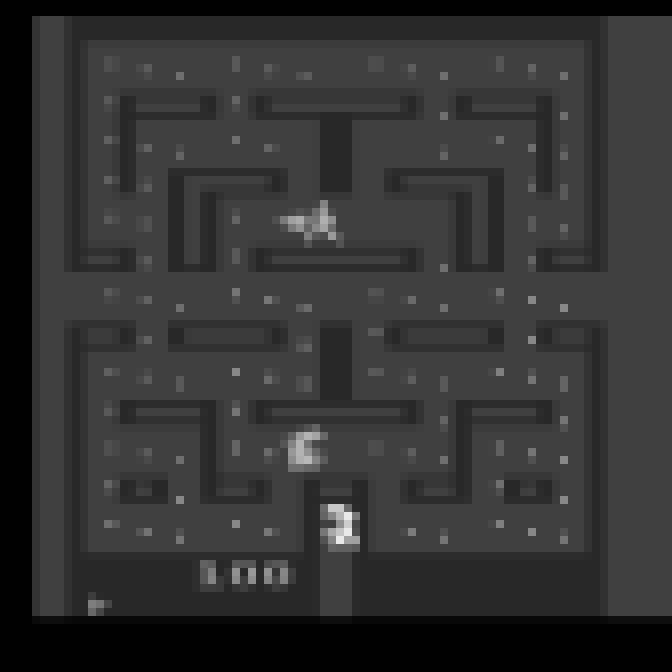
\includegraphics[width=\textwidth]{figures/atari.png}
    \caption{The \textsc{Alien-v5} environment is an example of the \textsc{Atari} games consisting of a maze filled with 'eggs' to destroy while being hunted by aliens. A flamethrower or occasional power-up may be used to scare the aliens.}
    \label{fig:sample-env-atari}
  \end{subfigure}
  \hfill
  \begin{subfigure}[b]{0.32\textwidth}
    \centering
    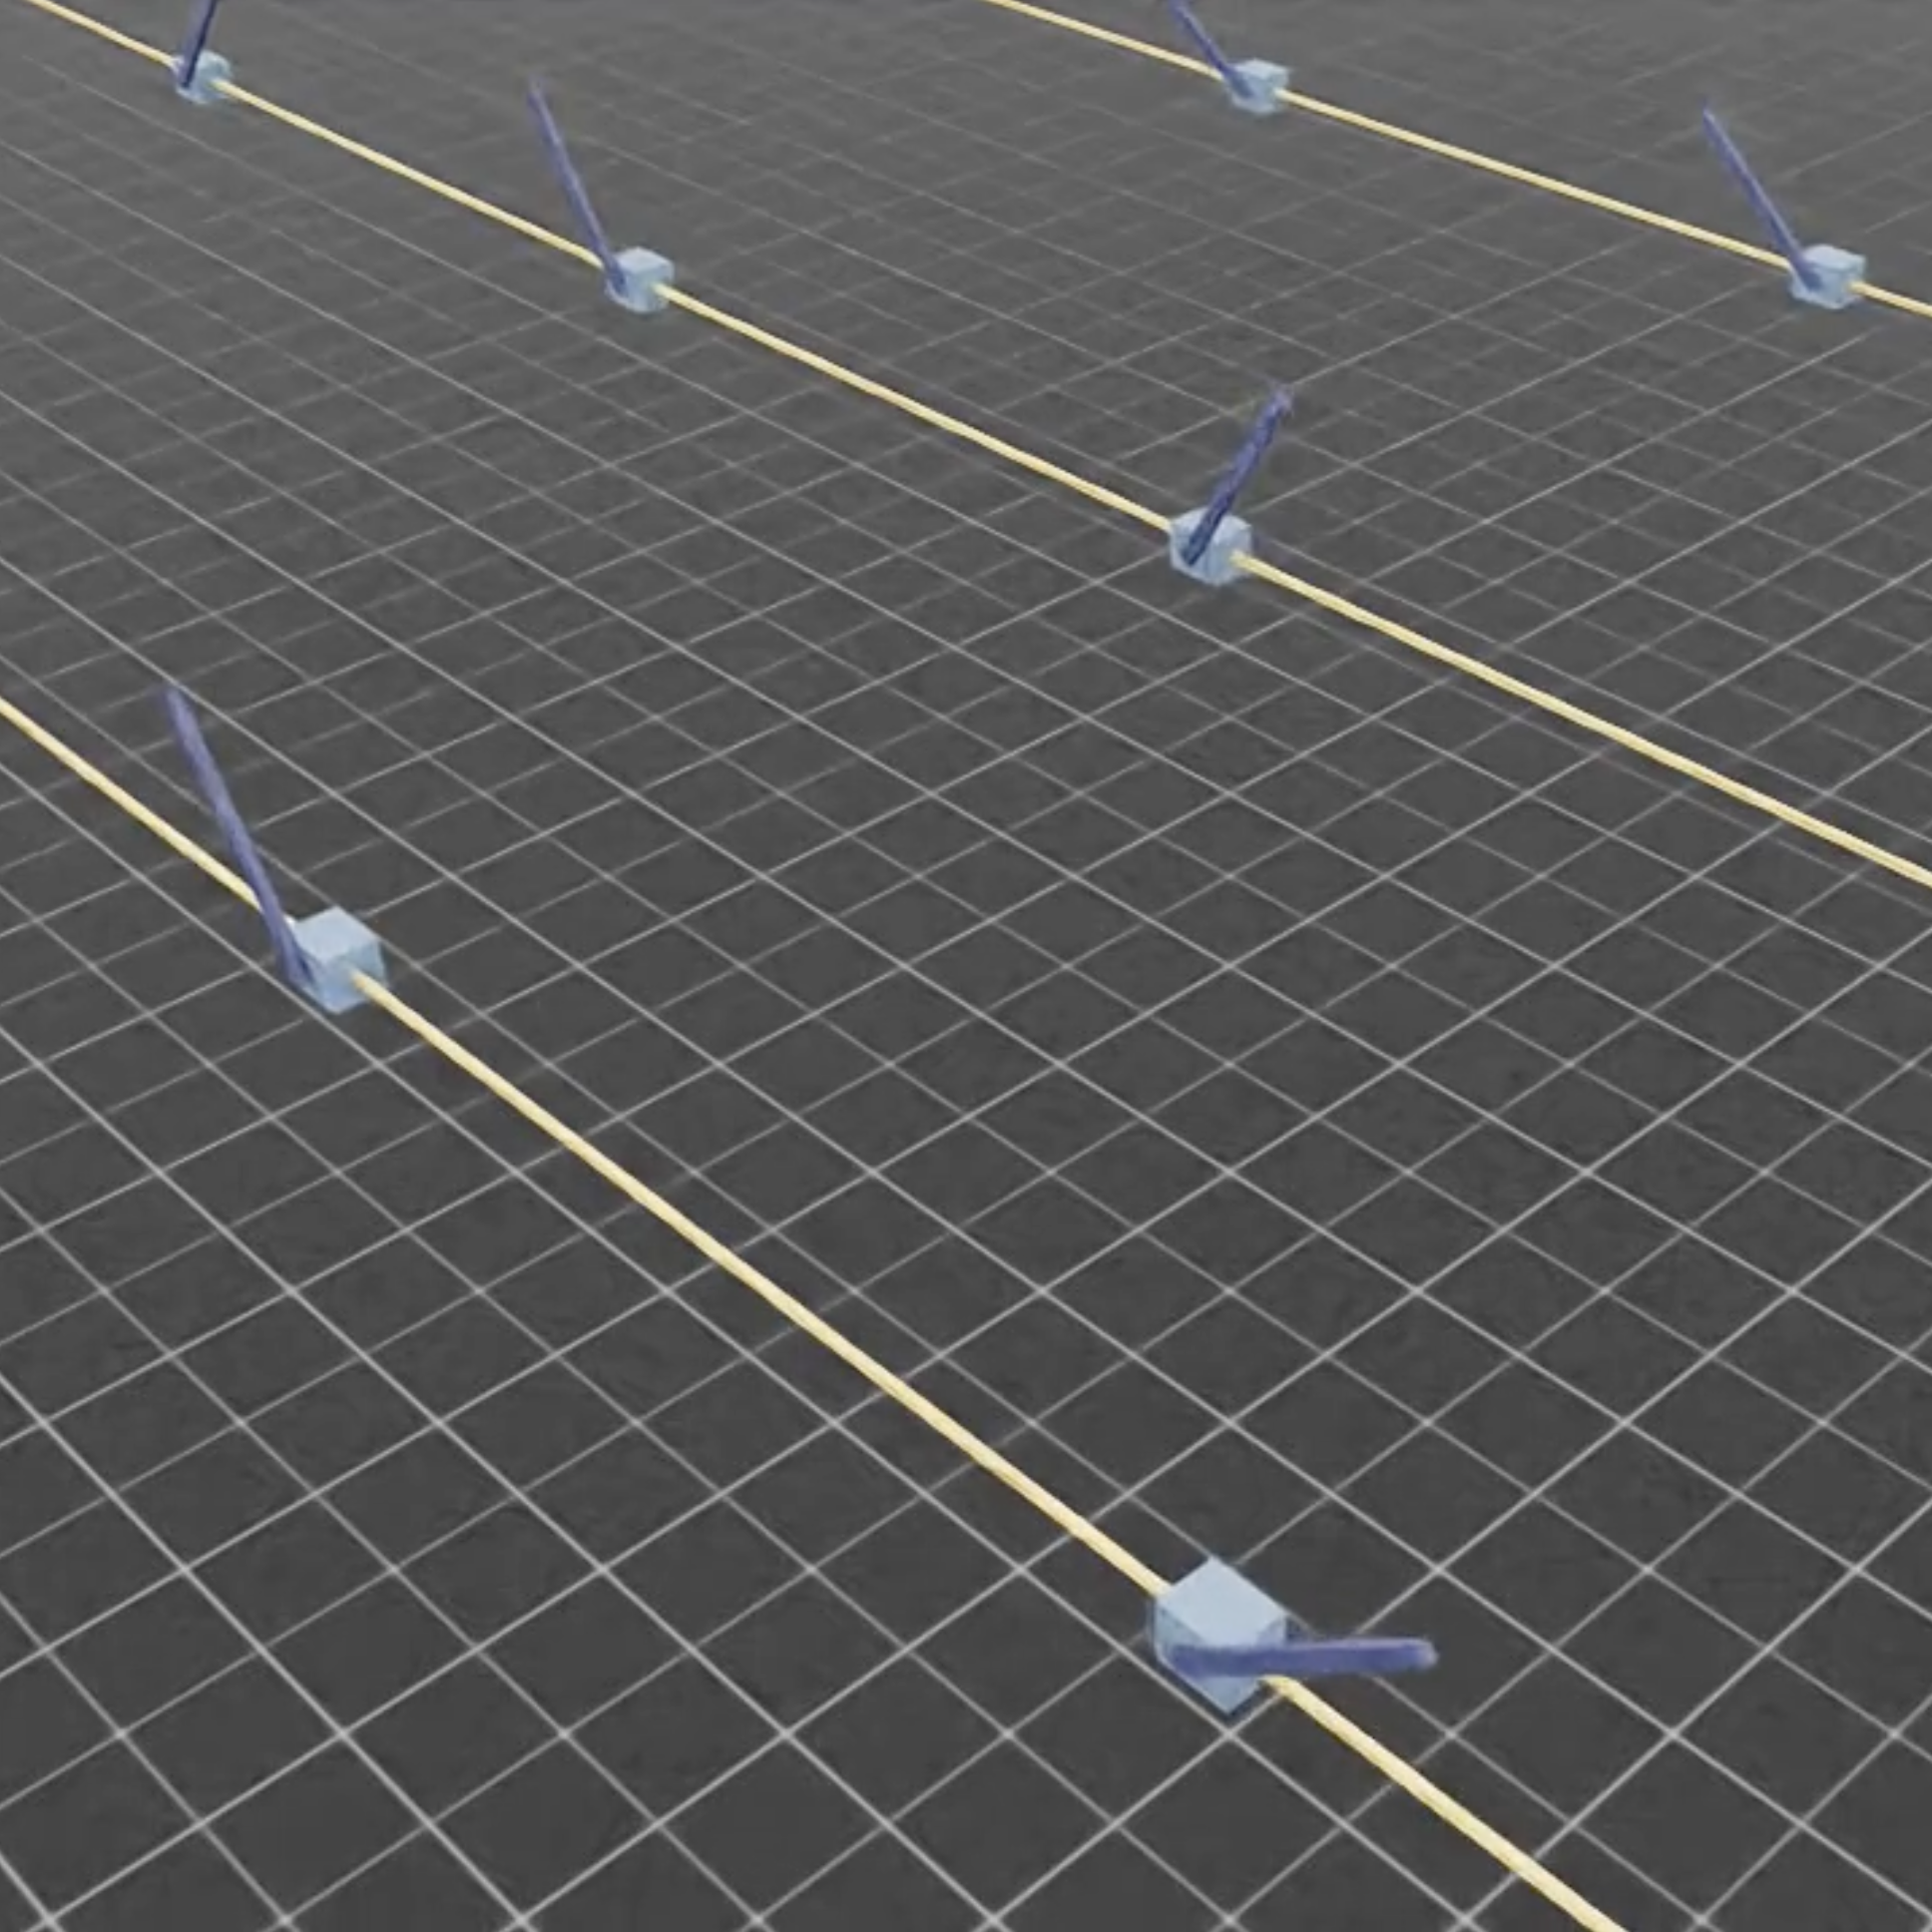
\includegraphics[width=\textwidth]{figures/isaac.png}
    \caption{The \textsc{CartPole} environment is an example of the \textsc{IsaacGym} environment.\\\textcolor{red}{What does the agent actually perceive?}\\}
    \label{fig:sample-env-isaac}
  \end{subfigure}
  \caption{Examples of the environments in use.}
  \label{fig:environmnents}
\end{figure}

\texttt{Include a description of how the experiments were set up that's clear enough a reader could replicate the setup.}
\texttt{Include a description of the specific measure used to evaluate the experiments (e.g. accuracy, precision@K, BLEU score, etc.).}
\texttt{Provide a link to your code or notebook (if available). Add in this section (or in the following) any reference to cloud-based providers you}

\subsection{Computational requirements}

\noindent The code for the \textsc{FourRoom} experiments was exclusively run on the CPU. For Atari, we experimented with the CPU, T4 GPU and TPU v2-8 in Google Colab. Weights \& Biases (wandb) was used for easier runtime visualization of the scores and other measures.

\noindent We would like to note, however, that \cite{rle-paper} had available the HPC resources of the MIT Supercloud and the Lincoln Laboratory Supercomputing Center. Within the framework of this course, we did not have the equivalent computing power to replicate all experiments in their original form and had to restrain ourselves to a mere few of them.

\texttt{Include a description of the hardware used, such as the GPU or CPU the experiments were run on. 
For each model, include a measure of the average runtime (e.g. average time to predict labels for a given validation set with a particular batch size).
For each experiment, include the total computational requirements (e.g. the total GPU hours spent).}\\
\texttt{Note: You'll likely have to record this as you run your experiments, so it's better to think about it ahead of time.}

\hypertarget{sec4}{\section{Results}}
\texttt{Start with a high-level overview of your results. Do your results support the main claims of the original paper? Keep this section as factual and precise as possible, and reserve your judgment and discussion points for the next "Discussion" section.}


\subsection{Results reproducing original paper}
\texttt{For each experiment, say (1) which claim in Section~\ref{sec:claims} it supports, and (2) if it successfully reproduced the associated experiment in the original paper.}
\texttt{For example, an experiment training and evaluating a model on a dataset may support a claim that that model outperforms some baseline.}
\texttt{Logically group related results into subsections.}

\subsubsection{Result 1}
\subsubsection{Result 2}

\subsection{Results beyond original paper}
\texttt{Often papers don't include enough information to fully specify their experiments, so some additional experimentation may be necessary. For example, it might be the case that batch size was not specified, and so different batch sizes need to be evaluated to reproduce the original results. Include the results of any additional experiments here. Note: this won't be necessary for all reproductions.}
 
\subsubsection{Additional Result 1}
\subsubsection{Additional Result 2}

\section{Discussion}

\texttt{Give your judgment on if your experimental results support the claims of the paper. Discuss the strengths and weaknesses of your approach - perhaps you didn't have time to run all the experiments, or perhaps you did additional experiments that further strengthened the claims in the paper.}

\subsection{What was easy}
Atari code was ready to run. 

\texttt{Give your judgment of what was easy to reproduce. Perhaps the author's code is clearly written and easy to run, so it was easy to verify the majority of original claims. Or, the explanation in the paper was really easy to follow and put into code.}

\texttt{Be careful not to give sweeping generalizations. Something that is easy for you might be difficult for others. Put what was easy in context and explain why it was easy (e.g. code had extensive API documentation and a lot of examples that matched experiments in papers).}

\subsection{What was difficult}
\begin{itemize}
  \item Isaac deprecated 
  \item FourRoom env missing
  \item Inconsistencies in the paper and lack of descriptions
  \item Hardware constraints`'
  \item Discrepancy between paper and code
\end{itemize}
\texttt{List part of the reproduction study that took more time than you anticipated or you felt was difficult.}

\texttt{Be careful to put your discussion in context. For example, don't say "The maths was difficult to follow", say "The math requires advanced knowledge of calculus to follow".}

\subsection{Communication with original authors}
\texttt{Document the extent of (or lack of) communication with the original authors. To make sure the reproducibility report is a fair assessment of the original research we recommend getting in touch with the original authors. We advise you to contact them through their email displayed in the paper and by asking specific questions.}

\section{Conclusion}
\texttt{Try to summarize the achievements of your project and its limits, suggesting (when appropriate) possible extensions and future works.}

\section*{Member contributions}
We send him an email got answer.

\texttt{Include a section specifying how you organized the work within the group and clearly describe the contributions of each member. Make sure to properly balance the workload among the members.}

%%%%

\bibliography{main}
\bibliographystyle{tmlr}

\appendix
\section{Appendix}
You may include other additional sections here. Here we provide suggestions and instructions for the layout and styling of the report.

\section{Citations, figures, and tables}

\paragraph{Citations}

When the authors or the publication are
included in the sentence, the citation should not be in parenthesis, using \verb|\citet{}| (as
in ``See \citet{Hinton06} for more information.''). Otherwise, the citation
should be in parenthesis using \verb|\citep{}| (as in ``Deep learning shows promise to make progress
towards AI~\citep{Bengio+chapter2007}.'').

\paragraph{Figures}

All artwork must be neat, clean, and legible. The figure number and caption always appear after the figure. Place one line space before the figure caption, and one line space after the figure. The figure caption is lowercase (except for the first word and proper nouns). Make sure the figure caption does not get separated from the figure. Leave sufficient space to avoid splitting the figure and figure caption.

\begin{figure}[ht]
\begin{center}
\fbox{\rule[-.5cm]{0cm}{4cm} \rule[-.5cm]{4cm}{0cm}}
\end{center}
\caption{Sample figure caption.}
\end{figure}

\paragraph{Tables}

All tables must be centered, neat, clean and legible. The table number and title always appear before the table. See Table~\ref{sample-table}. Place one line space before the table title, one line space after the table title, and one line space after the table. The table title must be lowercase (except for the first word and proper nouns).

\begin{table}[ht]
\caption{Sample table title}
\label{sample-table}
\begin{center}
\begin{tabular}{ll}
\multicolumn{1}{c}{\bf PART}  &\multicolumn{1}{c}{\bf DESCRIPTION}
\\ \hline \\
Dendrite         &Input terminal \\
Axon             &Output terminal \\
Soma             &Cell body (contains cell nucleus) \\
\end{tabular}
\end{center}
\end{table}

\section{Math Notation}

In an attempt to encourage standardized notation, we have included the
notation file from the textbook, \textit{Deep Learning}
\cite{goodfellow2016deep} available at
\url{https://github.com/goodfeli/dlbook_notation/}.  Use of this style
is not required and can be disabled by commenting out
\texttt{math\_commands.tex}.
\clearpage

\centerline{\bf Numbers and Arrays}
\bgroup
\def\arraystretch{1.5}
\begin{tabular}{p{1in}p{3.25in}}
$\displaystyle a$ & A scalar (integer or real)\\
$\displaystyle \va$ & A vector\\
$\displaystyle \mA$ & A matrix\\
$\displaystyle \tA$ & A tensor\\
$\displaystyle \mI_n$ & Identity matrix with $n$ rows and $n$ columns\\
$\displaystyle \mI$ & Identity matrix with dimensionality implied by context\\
$\displaystyle \ve^{(i)}$ & Standard basis vector $[0,\dots,0,1,0,\dots,0]$ with a 1 at position $i$\\
$\displaystyle \text{diag}(\va)$ & A square, diagonal matrix with diagonal entries given by $\va$\\
$\displaystyle \ra$ & A scalar random variable\\
$\displaystyle \rva$ & A vector-valued random variable\\
$\displaystyle \rmA$ & A matrix-valued random variable\\
\end{tabular}
\egroup
\vspace{0.25cm}

\centerline{\bf Sets and Graphs}
\bgroup
\def\arraystretch{1.5}

\begin{tabular}{p{1.25in}p{3.25in}}
$\displaystyle \sA$ & A set\\
$\displaystyle \R$ & The set of real numbers \\
$\displaystyle \{0, 1\}$ & The set containing 0 and 1 \\
$\displaystyle \{0, 1, \dots, n \}$ & The set of all integers between $0$ and $n$\\
$\displaystyle [a, b]$ & The real interval including $a$ and $b$\\
$\displaystyle (a, b]$ & The real interval excluding $a$ but including $b$\\
$\displaystyle \sA \backslash \sB$ & Set subtraction, i.e., the set containing the elements of $\sA$ that are not in $\sB$\\
$\displaystyle \gG$ & A graph\\
$\displaystyle \parents_\gG(\ervx_i)$ & The parents of $\ervx_i$ in $\gG$
\end{tabular}
\egroup
\vspace{0.25cm}

\clearpage
\centerline{\bf Indexing}
\bgroup
\def\arraystretch{1.5}

\begin{tabular}{p{1.25in}p{3.25in}}
$\displaystyle \eva_i$ & Element $i$ of vector $\va$, with indexing starting at 1 \\
$\displaystyle \eva_{-i}$ & All elements of vector $\va$ except for element $i$ \\
$\displaystyle \emA_{i,j}$ & Element $i, j$ of matrix $\mA$ \\
$\displaystyle \mA_{i, :}$ & Row $i$ of matrix $\mA$ \\
$\displaystyle \mA_{:, i}$ & Column $i$ of matrix $\mA$ \\
$\displaystyle \etA_{i, j, k}$ & Element $(i, j, k)$ of a 3-D tensor $\tA$\\
$\displaystyle \tA_{:, :, i}$ & 2-D slice of a 3-D tensor\\
$\displaystyle \erva_i$ & Element $i$ of the random vector $\rva$ \\
\end{tabular}
\egroup
\vspace{0.25cm}


\centerline{\bf Calculus}
\bgroup
\def\arraystretch{1.5}
\begin{tabular}{p{1.25in}p{3.25in}}
% NOTE: the [2ex] on the next line adds extra height to that row of the table.
% Without that command, the fraction on the first line is too tall and collides
% with the fraction on the second line.
$\displaystyle\frac{d y} {d x}$ & Derivative of $y$ with respect to $x$\\ [2ex]
$\displaystyle \frac{\partial y} {\partial x} $ & Partial derivative of $y$ with respect to $x$ \\
$\displaystyle \nabla_\vx y $ & Gradient of $y$ with respect to $\vx$ \\
$\displaystyle \nabla_\mX y $ & Matrix derivatives of $y$ with respect to $\mX$ \\
$\displaystyle \nabla_\tX y $ & Tensor containing derivatives of $y$ with respect to $\tX$ \\
$\displaystyle \frac{\partial f}{\partial \vx} $ & Jacobian matrix $\mJ \in \R^{m\times n}$ of $f: \R^n \rightarrow \R^m$\\
$\displaystyle \nabla_\vx^2 f(\vx)\text{ or }\mH( f)(\vx)$ & The Hessian matrix of $f$ at input point $\vx$\\
$\displaystyle \int f(\vx) d\vx $ & Definite integral over the entire domain of $\vx$ \\
$\displaystyle \int_\sS f(\vx) d\vx$ & Definite integral with respect to $\vx$ over the set $\sS$ \\
\end{tabular}
\egroup
\vspace{0.25cm}

\centerline{\bf Probability and Information Theory}
\bgroup
\def\arraystretch{1.5}
\begin{tabular}{p{1.25in}p{3.25in}}
$\displaystyle P(\ra)$ & A probability distribution over a discrete variable\\
$\displaystyle p(\ra)$ & A probability distribution over a continuous variable, or over
a variable whose type has not been specified\\
$\displaystyle \ra \sim P$ & Random variable $\ra$ has distribution $P$\\% so thing on left of \sim should always be a random variable, with name beginning with \r
$\displaystyle  \E_{\rx\sim P} [ f(x) ]\text{ or } \E f(x)$ & Expectation of $f(x)$ with respect to $P(\rx)$ \\
$\displaystyle \Var(f(x)) $ &  Variance of $f(x)$ under $P(\rx)$ \\
$\displaystyle \Cov(f(x),g(x)) $ & Covariance of $f(x)$ and $g(x)$ under $P(\rx)$\\
$\displaystyle H(\rx) $ & Shannon entropy of the random variable $\rx$\\
$\displaystyle \KL ( P \Vert Q ) $ & Kullback-Leibler divergence of P and Q \\
$\displaystyle \mathcal{N} ( \vx ; \vmu , \mSigma)$ & Gaussian distribution %
over $\vx$ with mean $\vmu$ and covariance $\mSigma$ \\
\end{tabular}
\egroup
\vspace{0.25cm}

\clearpage
\centerline{\bf Functions}
\bgroup
\def\arraystretch{1.5}
\begin{tabular}{p{1.25in}p{3.25in}}
$\displaystyle f: \sA \rightarrow \sB$ & The function $f$ with domain $\sA$ and range $\sB$\\
$\displaystyle f \circ g $ & Composition of the functions $f$ and $g$ \\
  $\displaystyle f(\vx ; \vtheta) $ & A function of $\vx$ parametrized by $\vtheta$.
  (Sometimes we write $f(\vx)$ and omit the argument $\vtheta$ to lighten notation) \\
$\displaystyle \log x$ & Natural logarithm of $x$ \\
$\displaystyle \sigma(x)$ & Logistic sigmoid, $\displaystyle \frac{1} {1 + \exp(-x)}$ \\
$\displaystyle \zeta(x)$ & Softplus, $\log(1 + \exp(x))$ \\
$\displaystyle || \vx ||_p $ & $\normlp$ norm of $\vx$ \\
$\displaystyle || \vx || $ & $\normltwo$ norm of $\vx$ \\
$\displaystyle x^+$ & Positive part of $x$, i.e., $\max(0,x)$\\
$\displaystyle \1_\mathrm{condition}$ & is 1 if the condition is true, 0 otherwise\\
\end{tabular}
\egroup
\vspace{0.25cm}


\end{document}
